\documentclass[unicode,11pt,a4paper,oneside,numbers=endperiod,openany]{scrartcl}
\usepackage{graphicx}
\usepackage{subcaption}
\usepackage{mwe}
\usepackage{float}
\usepackage{amsmath}

\usepackage{ifthen}
\usepackage[utf8]{inputenc}
\usepackage{graphics}
\usepackage{graphicx}
\usepackage{hyperref}

\pagestyle{plain}
\voffset -5mm
\oddsidemargin  0mm
\evensidemargin -11mm
\marginparwidth 2cm
\marginparsep 0pt
\topmargin 0mm
\headheight 0pt
\headsep 0pt
\topskip 0pt        
\textheight 255mm
\textwidth 165mm

\newcommand{\duedate} {}
\newcommand{\setduedate}[1]{%
\renewcommand\duedate {Due date:~ #1}}
\newcommand\isassignment {false}
\newcommand{\setassignment}{\renewcommand\isassignment {true}}
\newcommand{\ifassignment}[1]{\ifthenelse{\boolean{\isassignment}}{#1}{}}
\newcommand{\ifnotassignment}[1]{\ifthenelse{\boolean{\isassignment}}{}{#1}}

\newcommand{\assignmentpolicy}{
\begin{table}[h]
\begin{center}
\scalebox{0.8} {%
\begin{tabular}{|p{0.02cm}p{16cm}|}
\hline
&\\
\multicolumn{2}{|c|}{\Large\textbf{HPC  2021 ---  Submission Instructions}}\\
\multicolumn{2}{|c|}{\large\textbf{(Please, notice that following instructions are mandatory: }}\\
\multicolumn{2}{|c|}{\large\textbf{submissions that don't comply with, won't be considered)}}\\
&\\
\textbullet & Assignments must be submitted to \href{https://www.icorsi.ch/course/view.php?id=14652}{iCorsi} (i.e. in electronic format).\\
\textbullet & Provide both executable package and sources (e.g. C/C++ files, Matlab). 
If you are using libraries, please add them in the file. Sources must be organized in directories called:\\
\multicolumn{2}{|c|}{\textit{Project\_number\_lastname\_firstname}}\\
& and  the  file must be called:\\
\multicolumn{2}{|c|}{\textit{project\_number\_lastname\_firstname.zip}}\\
\multicolumn{2}{|c|}{\textit{project\_number\_lastname\_firstname.pdf}}\\
\textbullet &  The TAs will grade your project by reviewing your project write-up, and looking at the implementation 
                 you attempted, and benchmarking your code's performance.\\

\textbullet & You are allowed to discuss all questions with anyone you like; however: (i) your submission must list anyone you discussed problems with and (ii) you must write up your submission independently.\\
\hline
\end{tabular}
}
\end{center}
\end{table}
}
\newcommand{\punkte}[1]{\hspace{1ex}\emph{\mdseries\hfill(#1~\ifcase#1{Points}\or{Points}\else{Points}\fi)}}


\newcommand\serieheader[6]{
\thispagestyle{empty}%
\begin{flushleft}

\includegraphics[width=0.4\textwidth]{usi_inf.png}
\end{flushleft}
  \noindent%
  {\large\ignorespaces{\textbf{#1}}\hspace{\fill}\ignorespaces{ \textbf{#2}}}\\ \\%
  {\large\ignorespaces #3 \hspace{\fill}\ignorespaces #4}\\
  \noindent%
  \bigskip
  \hrule\par\bigskip\noindent%
  \bigskip {\ignorespaces {\Large{\textbf{#5}}}
  \hspace{\fill}\ignorespaces \large \ifthenelse{\boolean{\isassignment}}{\duedate}{#6}}
  \hrule\par\bigskip\noindent%  \linebreak
 }

\makeatletter
\def\enumerateMod{\ifnum \@enumdepth >3 \@toodeep\else
      \advance\@enumdepth \@ne
      \edef\@enumctr{enum\romannumeral\the\@enumdepth}\list
      {\csname label\@enumctr\endcsname}{\usecounter
        {\@enumctr}%%%? the following differs from "enumerate"
	\topsep0pt%
	\partopsep0pt%
	\itemsep0pt%
	\def\makelabel##1{\hss\llap{##1}}}\fi}
\let\endenumerateMod =\endlist
\makeatother




\usepackage{textcomp}





\begin{document}


\setassignment
\setduedate{07.12.2022, 23:59}

\serieheader{High-Performance Computing}{2022}{Student: SIMONE TARENZI}{Discussed with: VEDANG NAIK, ISIN SU ECEVIT}{Solution for Project 6}{}
\newline



\section{Task: Install METIS 5.0.2, and the corresponding Matlab mex interface}

The code worked, but it switched the values between p1 and p2.


\section{Task:  Construct adjacency matrices
from connectivity data [10 points]}

First the table data from the .csv files is loaded into the local variables XX\_coords and XX\_adjacency, where XX stands for the initials of the corresponding country. Then the tables are converted into an array, so that they can be used to actually create and visualize the graphs thanks to the gplotg function, that takes the adjacency array and the coordinate array.
\newline
Finally, the data for each country is saved as a .mat file in the folder Countries\_Mat following the desired format.

\section{Task: Implement various graph partitioning algorithms [25 points]}


\begin{table}[H]
\caption{Bisection results}
\centering
\small
\begin{tabular}{l|r|r|r|r} \hline\hline 
Mesh             &  Coordinate           & Metis 5.0.2  & Spectral & Inertial  \\ \hline
mesh1e1          &   18          &       17      &      18    &       20    \\             
mesh2e1          &   37          &      37       &    39      &     47      \\ 
mesh3e1   &              19      &     19      &      26    &       19    \\ 
mesh3em5   &          19          &       19      &    26      &   19        \\ 
airfoil1   &            94        &     77        &     132     &      93     \\ 
netz4504\_dual   &         25            &       23      &    23      &    27       \\ 
stufe            &              16          &      16       &      16    &      16     \\ 
3elt            &           172             &    124         &     117     &     257      \\ 
barth4           &             206           &       97      &   127       &     208      \\ 
ukerbe1         &               32         &      27       &  32        &     28      \\ 
crack            &            353           &       201      &    233      &    384       \\ 
\hline \hline
\end{tabular}
\label{table:bisection}
\end{table}


As the data shows, the Metis bisection always uses the least amount of cuts to bisect the given mesh.

\section{Task: Recursively bisecting meshes [15 points]}
\begin{table}[H]
\caption{Edge-cut results for recursive bi-partitioning, 8 / 16 partitions}
\centering
\scalebox{0.85}{
\begin{tabular}{l|r|r|r|r|r} \hline\hline 
 Case            &  Spectral  &  Metis 5.0.2    & Coordinate & Inertial  \\ \hline   
 airfoil1        & 398 / 633 & 320 / 563 & 516 / 819 & 670 / 1081 \\ 
 netz4504\_dual         & 111 / 184 & 110 / 161 & 127 / 198 & 165 / 271 \\       
 stufe         & 128 / 238 & 107 / 194 & 123 / 227 & 320 / 606 \\   
 3elt            & 469 / 752 & 395 / 651 & 733 / 1168 & 814 / 1230 \\  
 barth4          & 550 / 841 & 405 / 689 & 875 / 1306 & 977 / 1492 \\   
 ukerbe1         & 398 / 695 & 128 / 224 & 225 / 374 & 340 / 499 \\  
 crack           & 883 / 1419 & 784 / 1290 & 1343 / 1860 & 1351 / 1884 \\   \hline \hline
\end{tabular}
}
\label{table:Rec_bisection}
\end{table}

    \begin{figure}[H]
        \centering
        \begin{subfigure}[b]{0.477\textwidth}
            \centering
            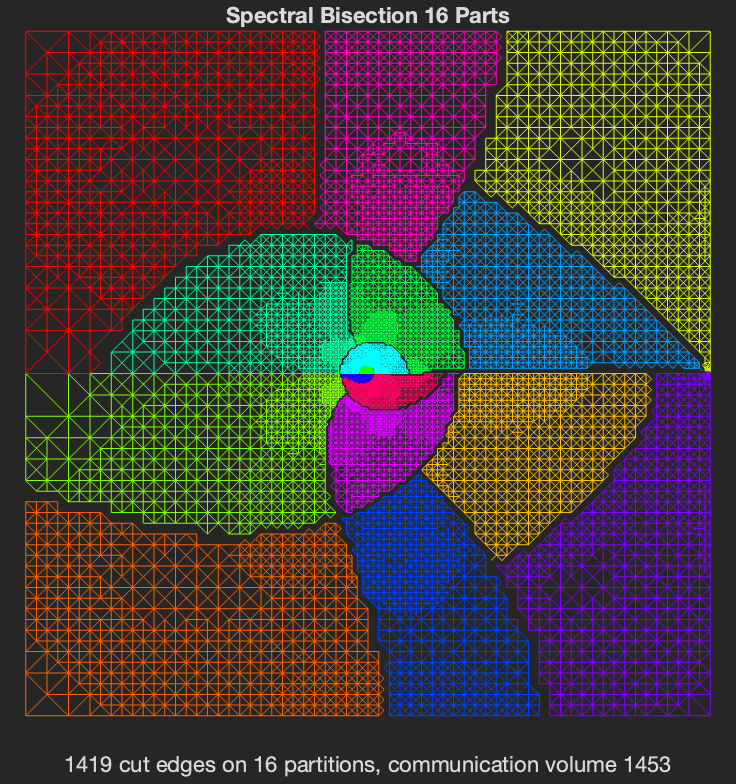
\includegraphics[width=\textwidth]{spec16.png}
            {{\small Spectral Bisection in 16 parts done on the "crack" mesh}}    
        \end{subfigure}
        \hfill
        \begin{subfigure}[b]{0.475\textwidth}  
            \centering 
            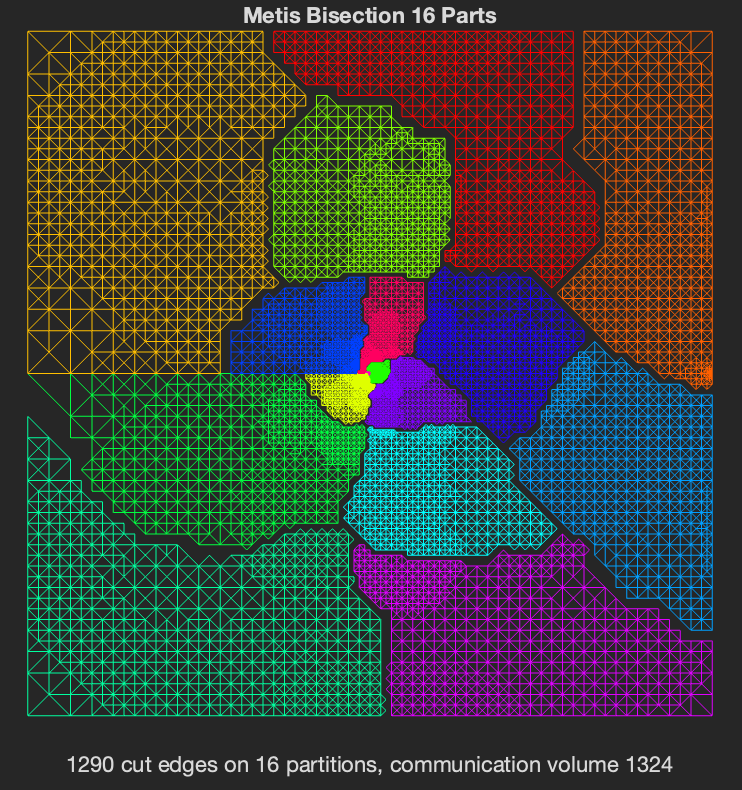
\includegraphics[width=\textwidth]{metis16.png}
            {{\small Metis Bisection in 16 parts done on the "crack" mesh}}    
        \end{subfigure}
        \vskip\baselineskip
        \begin{subfigure}[b]{0.487\textwidth}   
            \centering 
            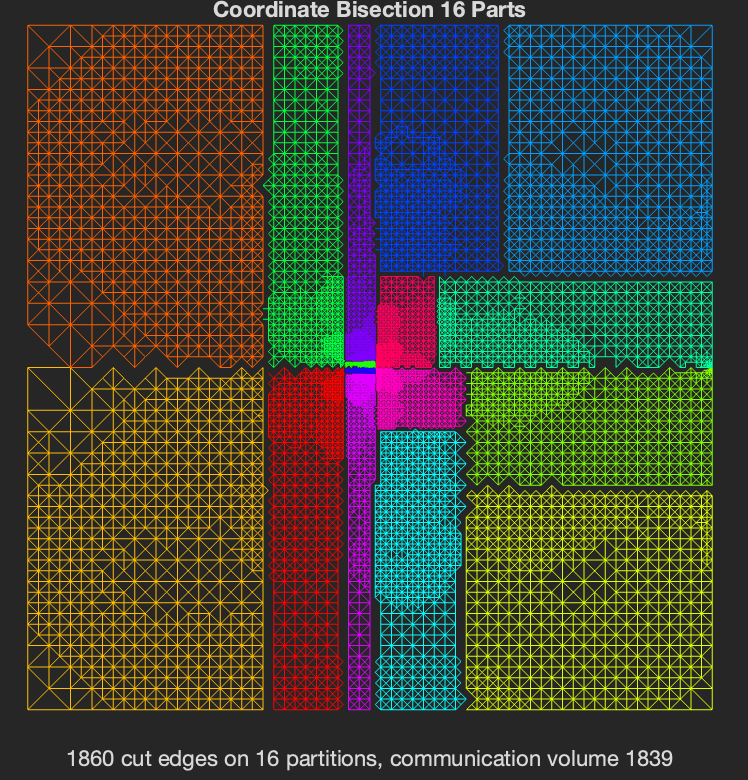
\includegraphics[width=\textwidth]{coord16.png}
            {{\small Coordinate Bisection in 16 parts done on the "crack" mesh}}    
        \end{subfigure}
        \hfill
        \begin{subfigure}[b]{0.475\textwidth}   
            \centering 
            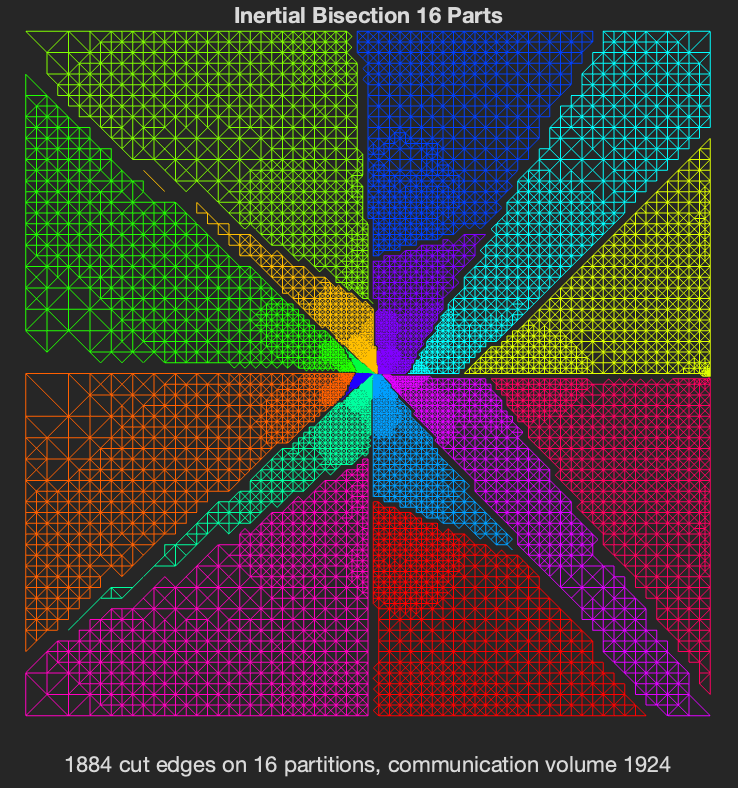
\includegraphics[width=\textwidth]{inert16.png}
            {{\small Inertial Bisection in 16 parts done on the "crack" mesh}}    
        \end{subfigure}
    \label{figure:crackmesh}
    \end{figure}


\section{Task: Comparing recursive bisection to direct $k$-way partitioning [10 points]}


\begin{table}[H]
\caption{Comparing the number of cut edges for recursive bisection and direct multiway partitioning in Metis 5.0.2.}
\begin{tabular}{l|r|r|r|r|r|r|r|}
\hline
Metis     & \multicolumn{1}{c|}{\begin{tabular}[c]{@{}c@{}}Luxemburg\\ 16 / 32\end{tabular}} & \multicolumn{1}{c|}{\begin{tabular}[c]{@{}c@{}}usroads-48\\ 16 / 32\end{tabular}} & \multicolumn{1}{c|}{\begin{tabular}[c]{@{}c@{}}Greece\\ 16 / 32\end{tabular}} & \multicolumn{1}{c|}{\begin{tabular}[c]{@{}c@{}}Switzerland\\ 16 / 32\end{tabular}} & \multicolumn{1}{c|}{\begin{tabular}[c]{@{}c@{}}Vietnam\\ 16 / 32\end{tabular}} & \multicolumn{1}{c|}{\begin{tabular}[c]{@{}c@{}}Norway\\ 16 / 32\end{tabular}} & \multicolumn{1}{c|}{\begin{tabular}[c]{@{}c@{}}Russia\\ 16 / 32\end{tabular}} \\ \hline
Recursive & 197 / 322                                                                        & 607 / 988                                                                         & 297 / 509                                                                     & 730 / 1089                                                                         & 245 / 445                                                                      & 284 / 470                                                                     & 616 / 1006                                                                    \\
Multiway  & 170 / 279                                                                        & 579 / 961                                                                         & 278 / 471                                                                     & 673 / 1042                                                                         & 245 / 411                                                                      & 255 / 439                                                                     & 551 / 933                                                                     \\ \hline
\end{tabular}
\end{table}

As the data shows, the Multiway Metis partitioning is always more conservative with the amount of cuts done compared to the recursive implementation.
\newline
This is working as expected: the recursive partitioning can be less optimal than the k-way one since it doesn't take into consideration the global information about the partitions. The k-way partitioning instead works on the whole graph by refining the partitioning at each step, and so the result can be way more efficient.

\begin{figure}[!ht]
        \centering
        \begin{subfigure}[b]{0.49\textwidth}
            \centering
            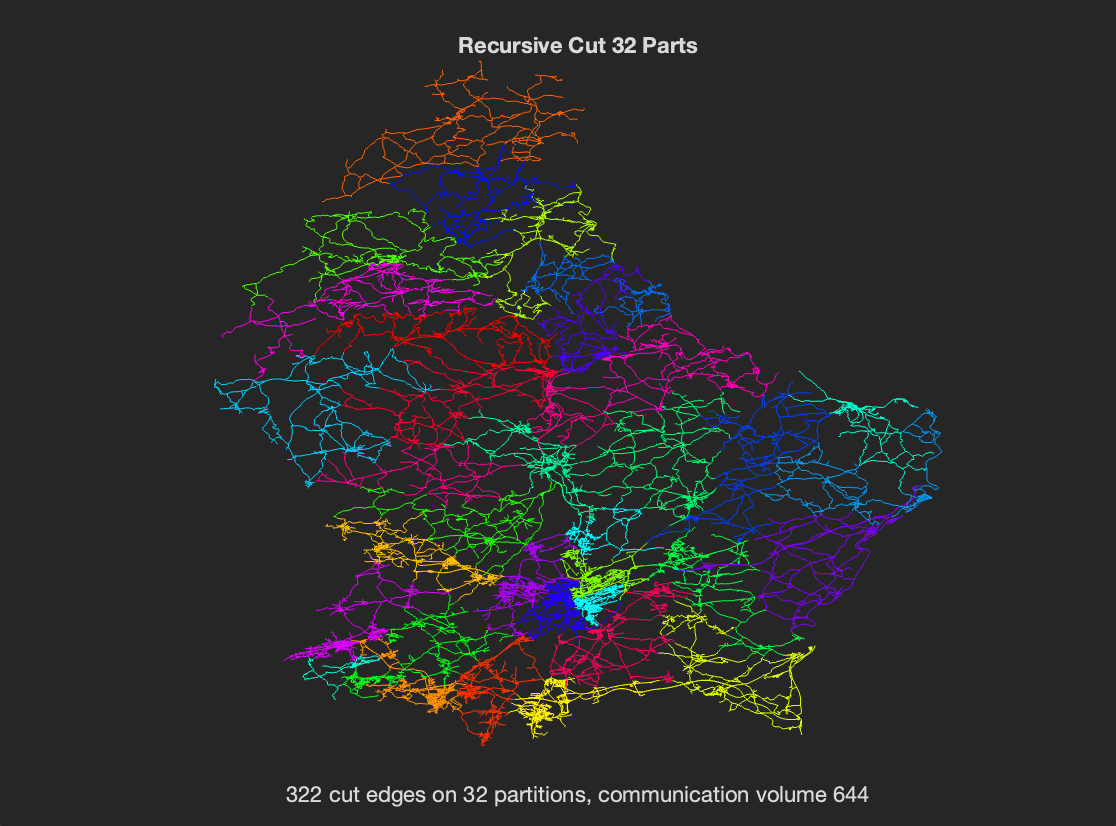
\includegraphics[width=\textwidth]{lux_rec.png}
            {{\small Recursive Metis bisection in 32 parts of the Luxembourg roads mesh}}    
        \end{subfigure}
        \hfill
        \begin{subfigure}[b]{0.49\textwidth}  
            \centering 
            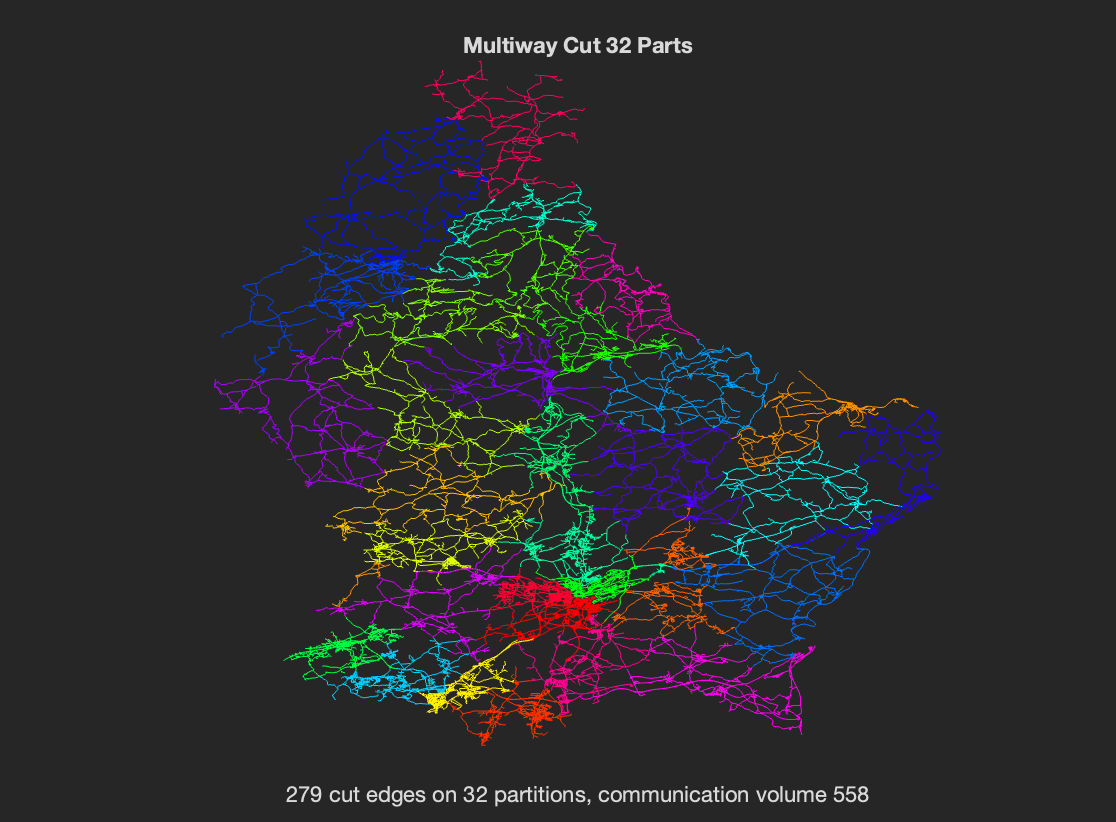
\includegraphics[width=\textwidth]{lux_kway.png}
            {{\small Multiway Metis partitioning in 32 parts of the Luxembourg roads mesh}}    
        \end{subfigure}
        \vskip\baselineskip
        \begin{subfigure}[b]{0.49\textwidth}   
            \centering 
            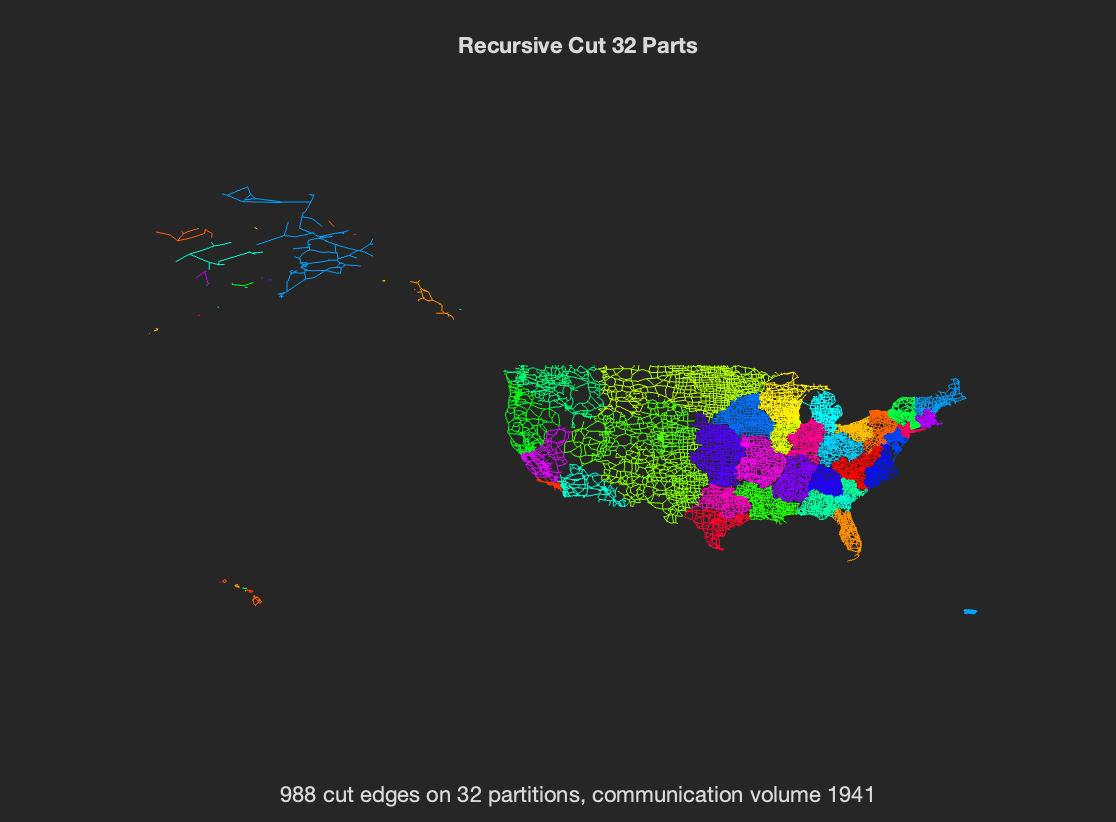
\includegraphics[width=\textwidth]{usa_rec.png}
            {{\small Recursive Metis bisection in 32 parts of the United States roads mesh}}    
        \end{subfigure}
        \hfill
        \begin{subfigure}[b]{0.49\textwidth}   
            \centering 
            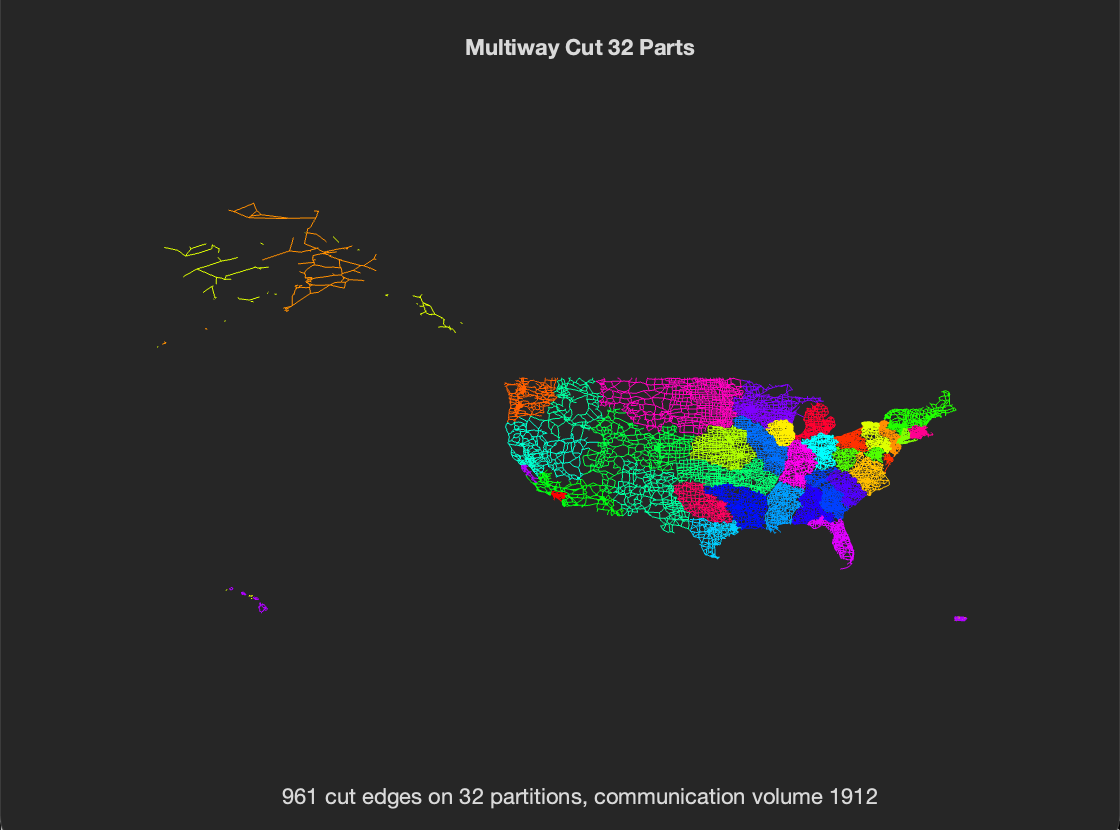
\includegraphics[width=\textwidth]{usa_kway.png}
            {{\small Multiway Metis partitioning in 32 parts of the United States roads mesh}}    
        \end{subfigure}
	\vskip\baselineskip
	\begin{subfigure}[b]{0.49\textwidth}   
            \centering 
            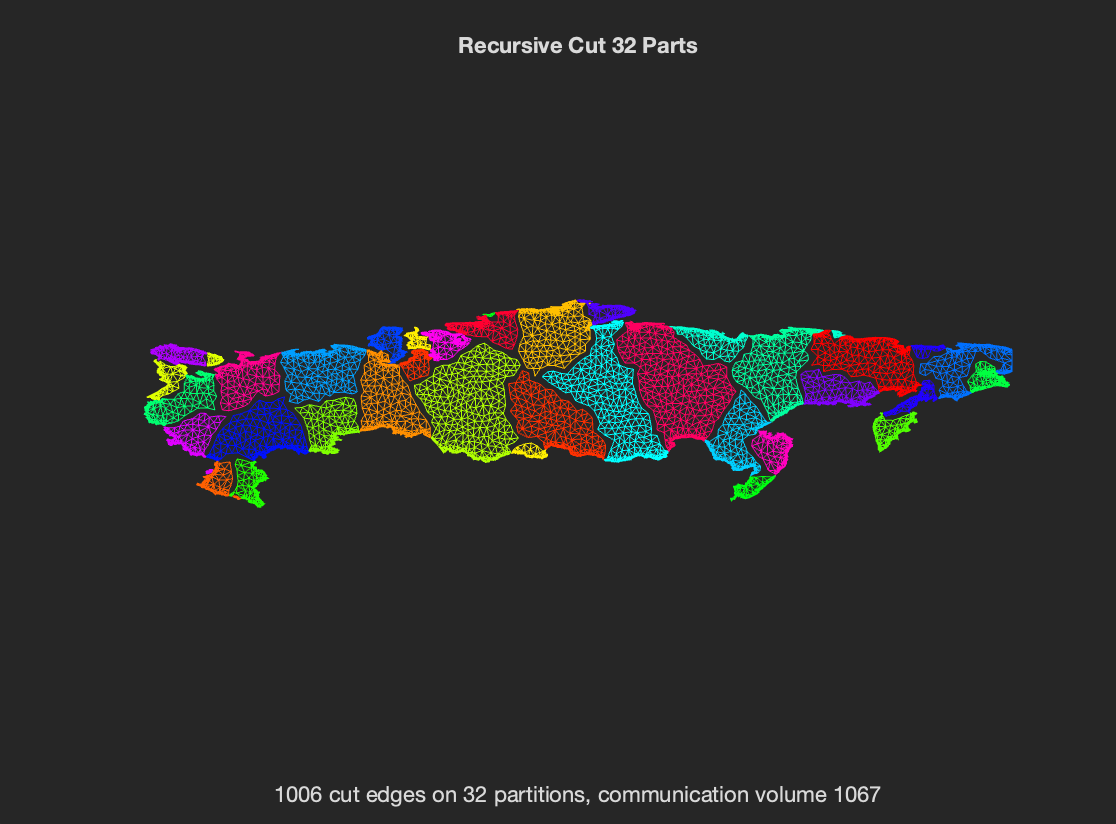
\includegraphics[width=\textwidth]{russia_rec.png}
            {{\small Recursive Metis bisection in 32 parts of the Russia map mesh}}    
        \end{subfigure} 
	\begin{subfigure}[b]{0.49\textwidth}   
            \centering 
            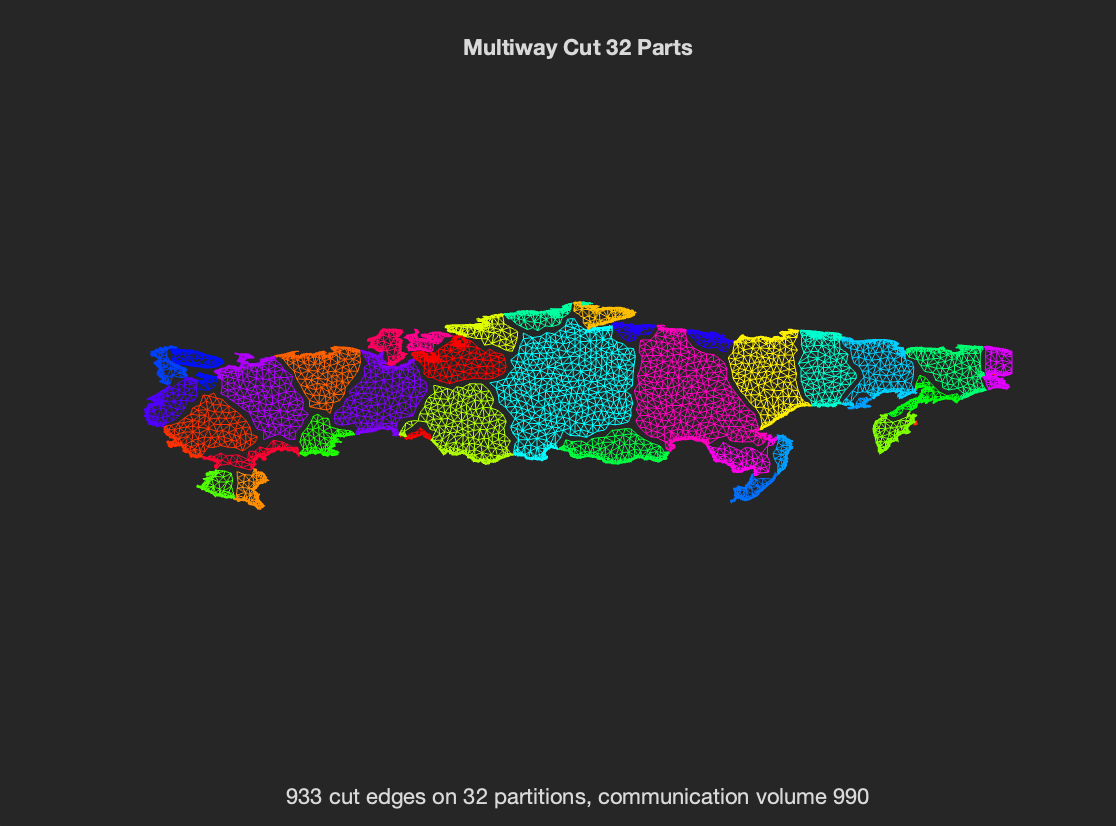
\includegraphics[width=\textwidth]{russia_kway.png}
            {{\small Multiway Metis partitioning in 32 parts of the Russia map mesh}}    
        \end{subfigure} 
    \label{figure:metismeshes}
    \end{figure}

\section{Task: Utilizing graph eigenvectors [25 points]}

\begin{figure}[H]
        \centering
        \begin{subfigure}[b]{0.475\textwidth}
            \centering
            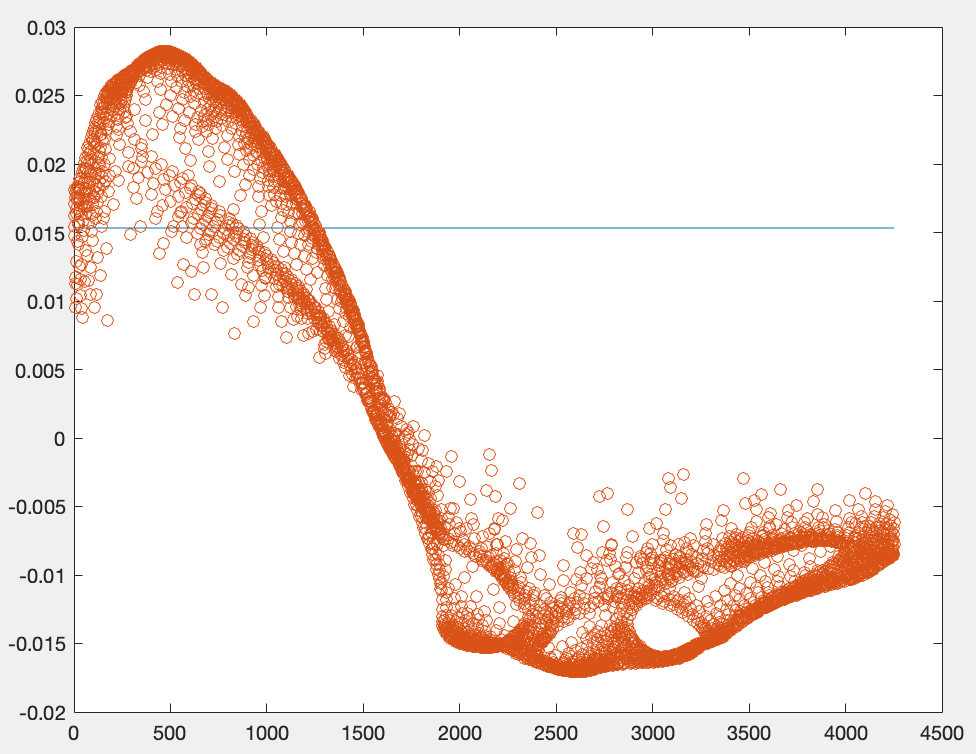
\includegraphics[width=\textwidth]{1.png}
            {{\small Entries of the eigenvectors associated with the first (blue) and second (red) smallest eigenvalues of the Laplacian matrix L for the graph ”airfoil1.”}}    
        \end{subfigure}
        \hfill
        \begin{subfigure}[b]{0.475\textwidth}  
            \centering 
            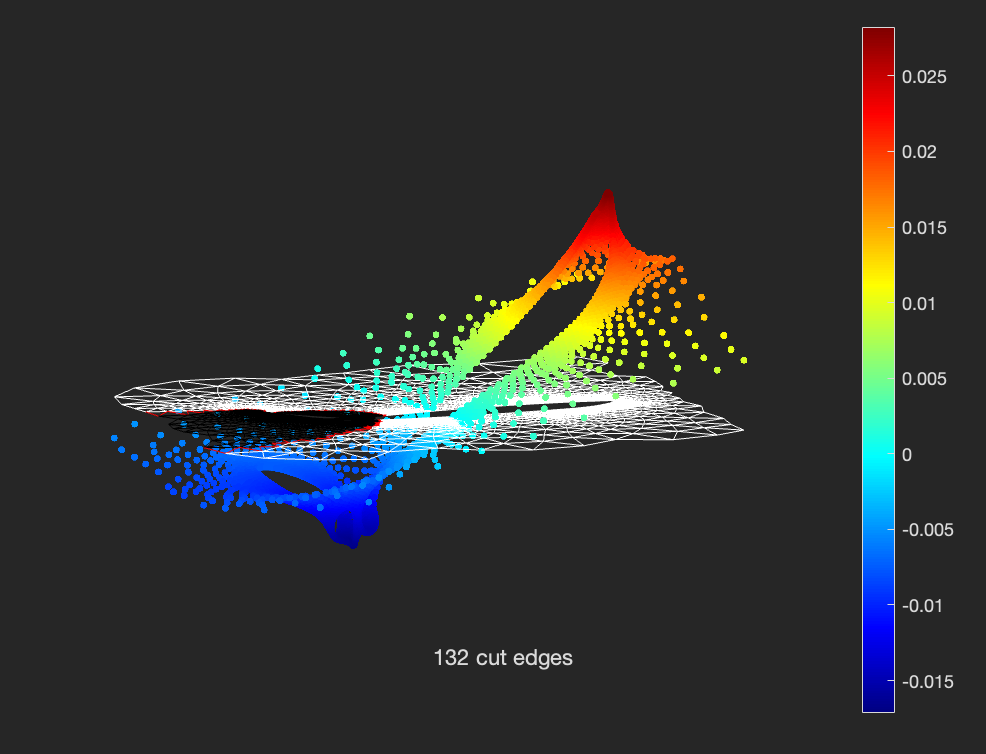
\includegraphics[width=\textwidth]{2.png}
            {{\small Projection of the entries of the eigenvector associated with the second smallest eigenvalue onto the coordinate system space of the graph ”airfoil1.”}}    
        \end{subfigure}
        \vskip\baselineskip
        \begin{subfigure}[b]{0.475\textwidth}   
            \centering 
            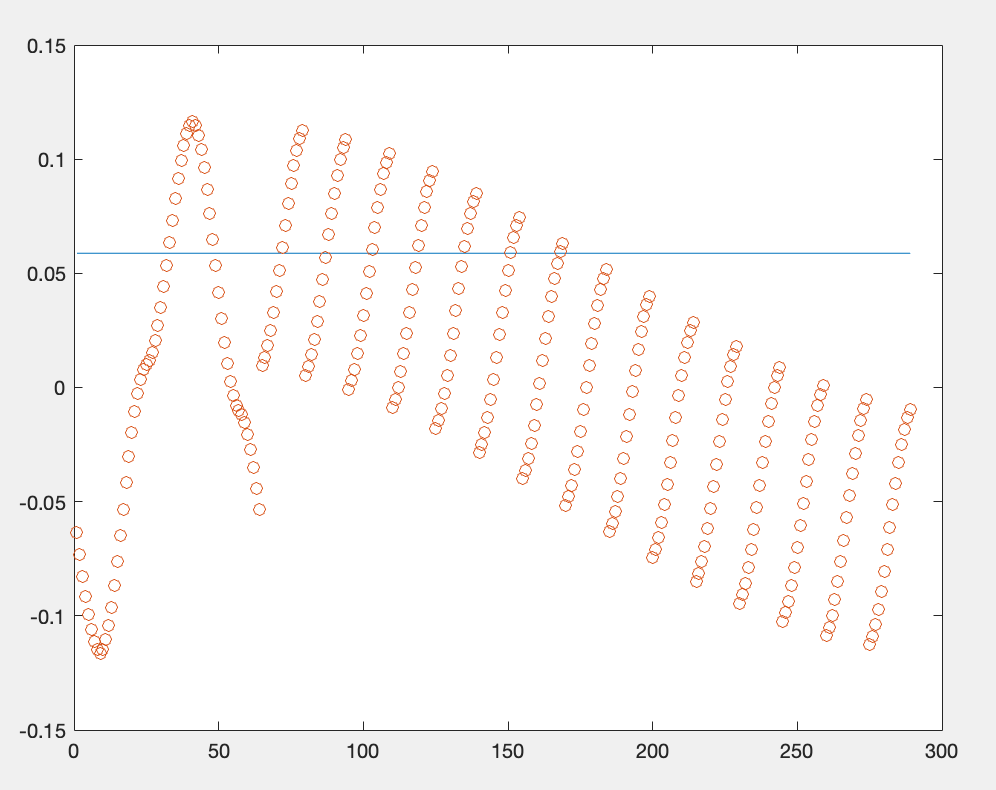
\includegraphics[width=\textwidth]{4.png}
            {{\small Entries of the eigenvectors associated with the first (blue) and second (red) smallest eigenvalues of the Laplacian matrix L for the graph ”mesh3e1.”}}    
        \end{subfigure}
        \hfill
        \begin{subfigure}[b]{0.475\textwidth}   
            \centering 
            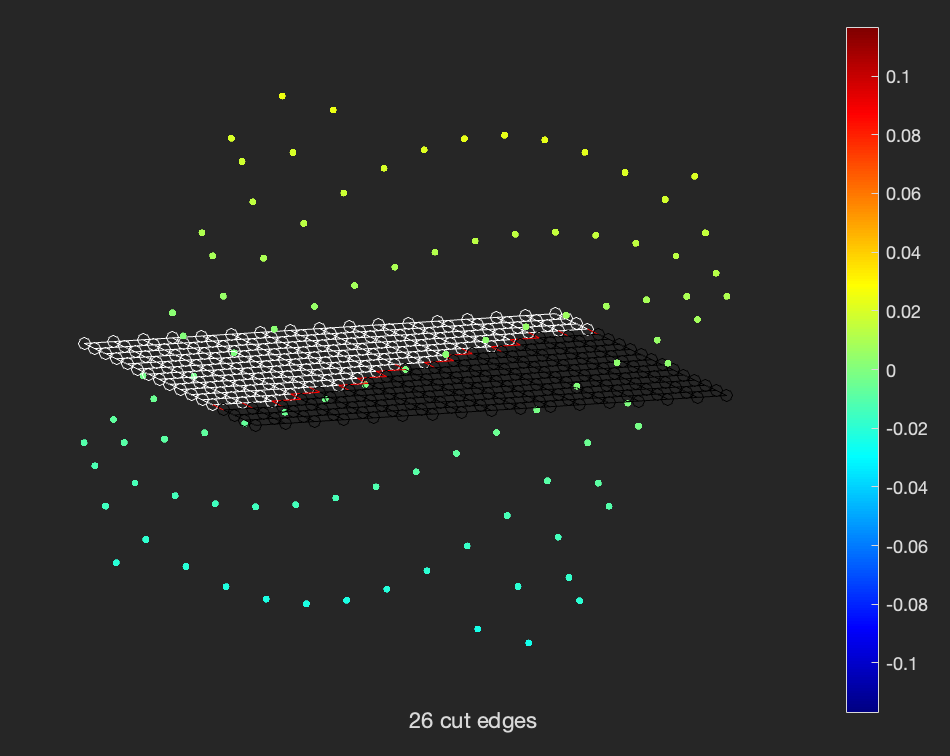
\includegraphics[width=\textwidth]{5.png}
            {{\small Projection of the entries of the eigenvector associated with the second smallest eigenvalue onto the coordinate system space of the graph ”mesh3e1.”}}    
        \end{subfigure}
\vskip\baselineskip
        \begin{subfigure}[b]{0.475\textwidth}   
            \centering 
            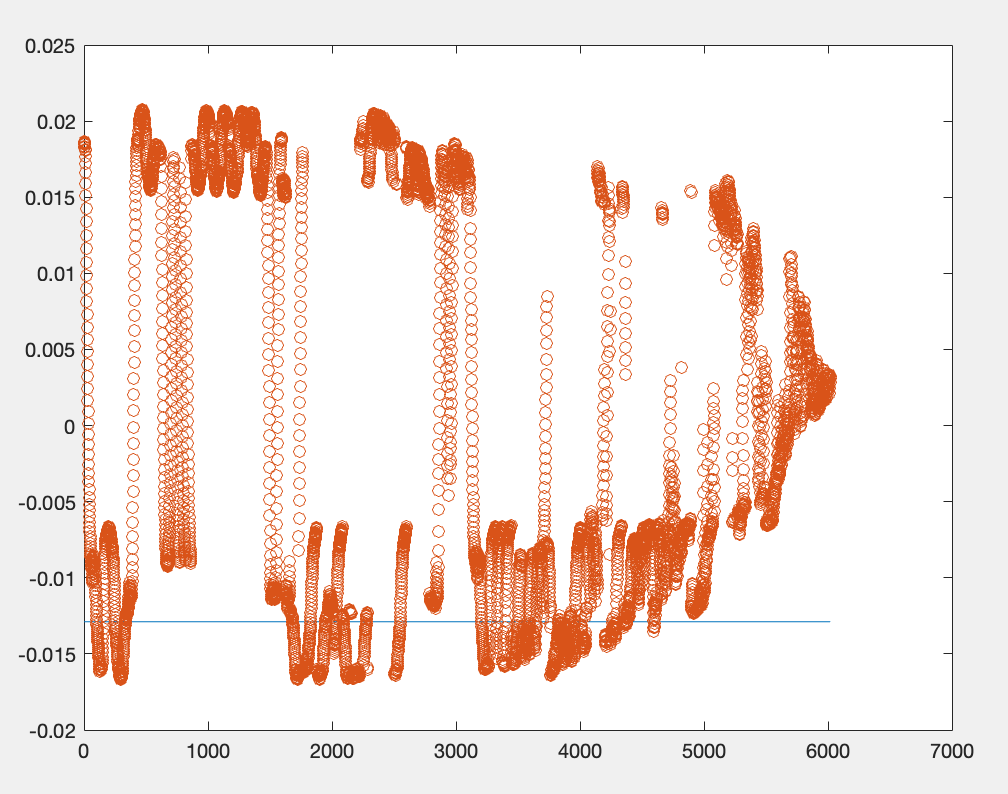
\includegraphics[width=\textwidth]{7.png}
            {{\small Entries of the eigenvectors associated with the first (blue) and second (red) smallest eigenvalues of the Laplacian matrix L for the graph ”barth4.”}}    
        \end{subfigure}
        \hfill
        \begin{subfigure}[b]{0.475\textwidth}   
            \centering 
            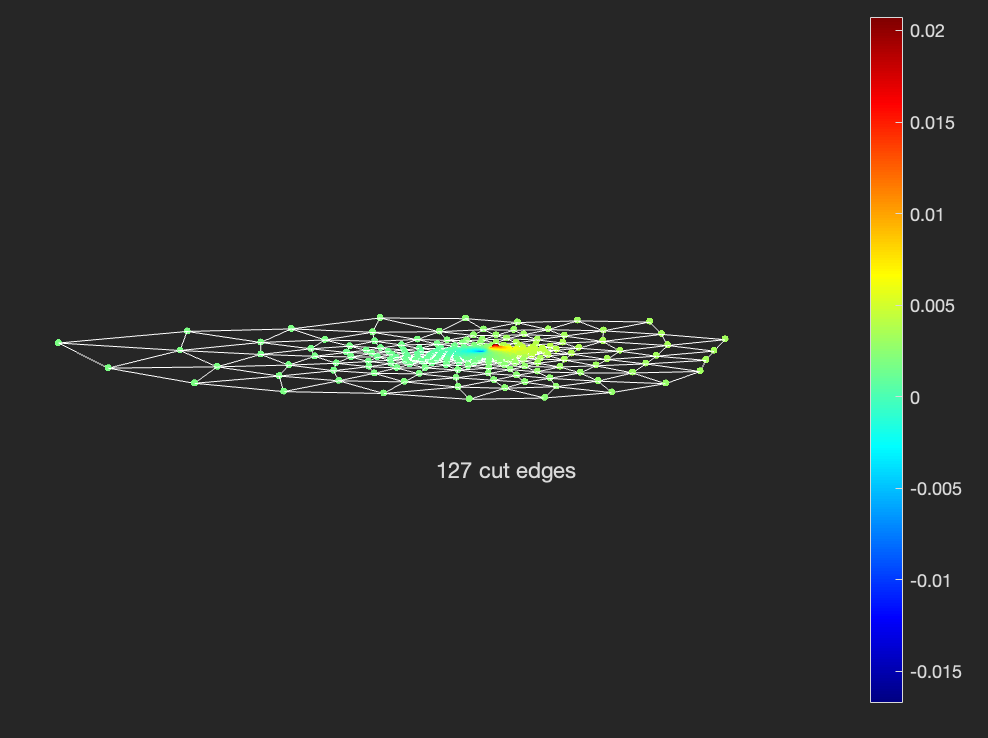
\includegraphics[width=\textwidth]{8.png}
            {{\small Projection of the entries of the eigenvector associated with the second smallest eigenvalue onto the coordinate system space of the graph ”barth4.”}}    
        \end{subfigure}
    \label{figure:ex6meshes}
    \end{figure}

\begin{figure}[H]
        \centering
\begin{subfigure}[b]{0.475\textwidth}   
            \centering 
            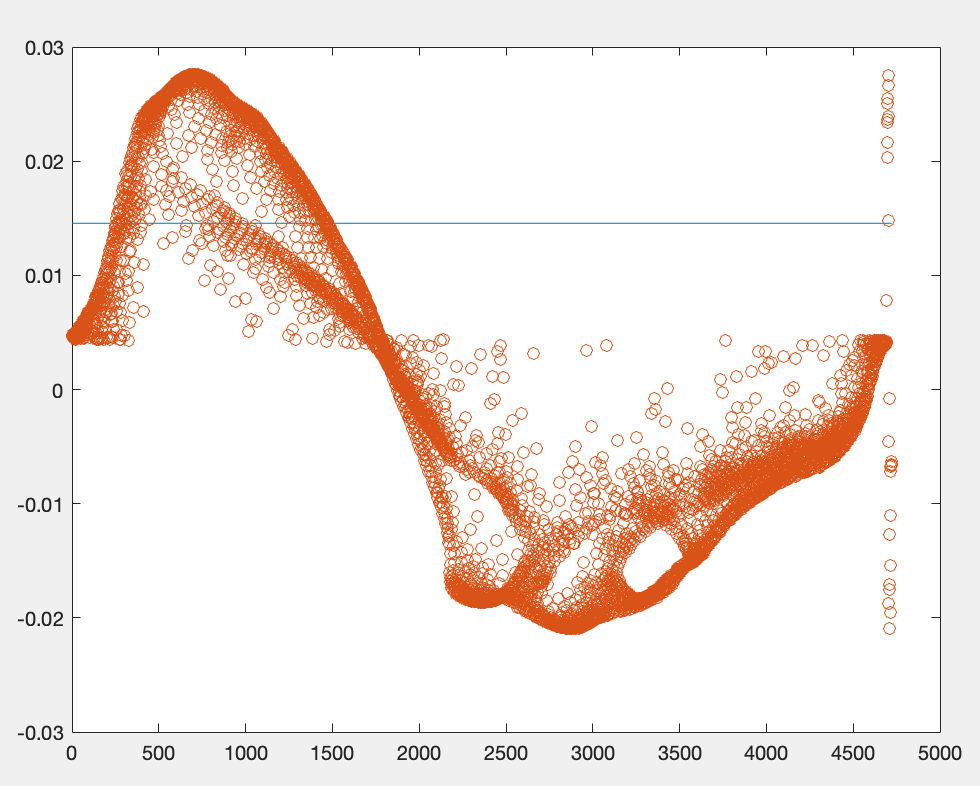
\includegraphics[width=\textwidth]{10.png}
            {{\small Entries of the eigenvectors associated with the first (blue) and second (red) smallest eigenvalues of the Laplacian matrix L for the graph ”3elt.”}}    
        \end{subfigure}
        \hfill
        \begin{subfigure}[b]{0.475\textwidth}   
            \centering 
            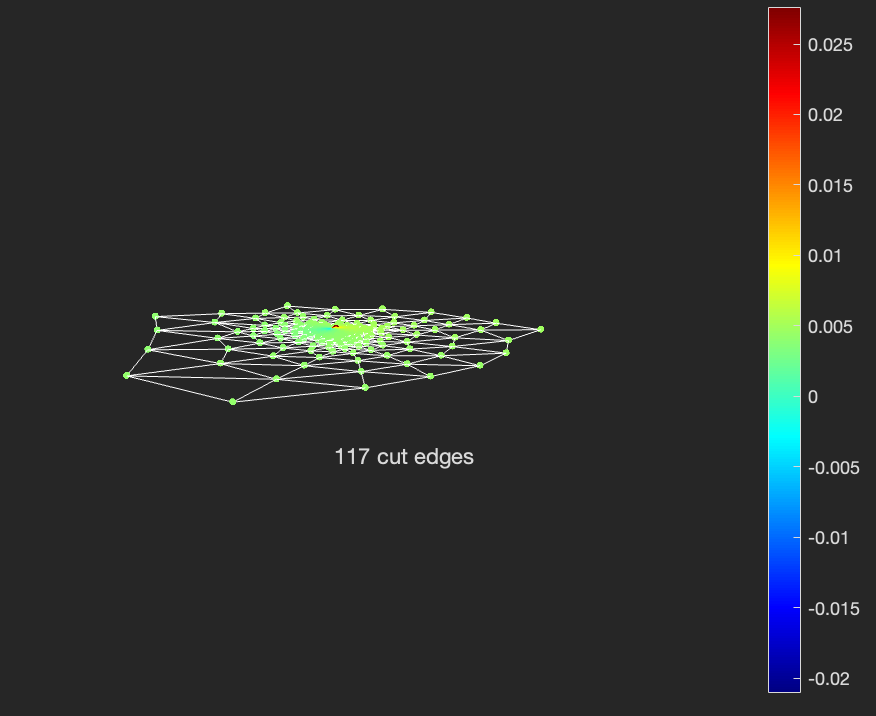
\includegraphics[width=\textwidth]{11.png}
            {{\small Projection of the entries of the eigenvector associated with the second smallest eigenvalue onto the coordinate system space of the graph ”3elt.”}}    
        \end{subfigure}
\vskip\baselineskip
        \begin{subfigure}[b]{0.475\textwidth}   
            \centering 
            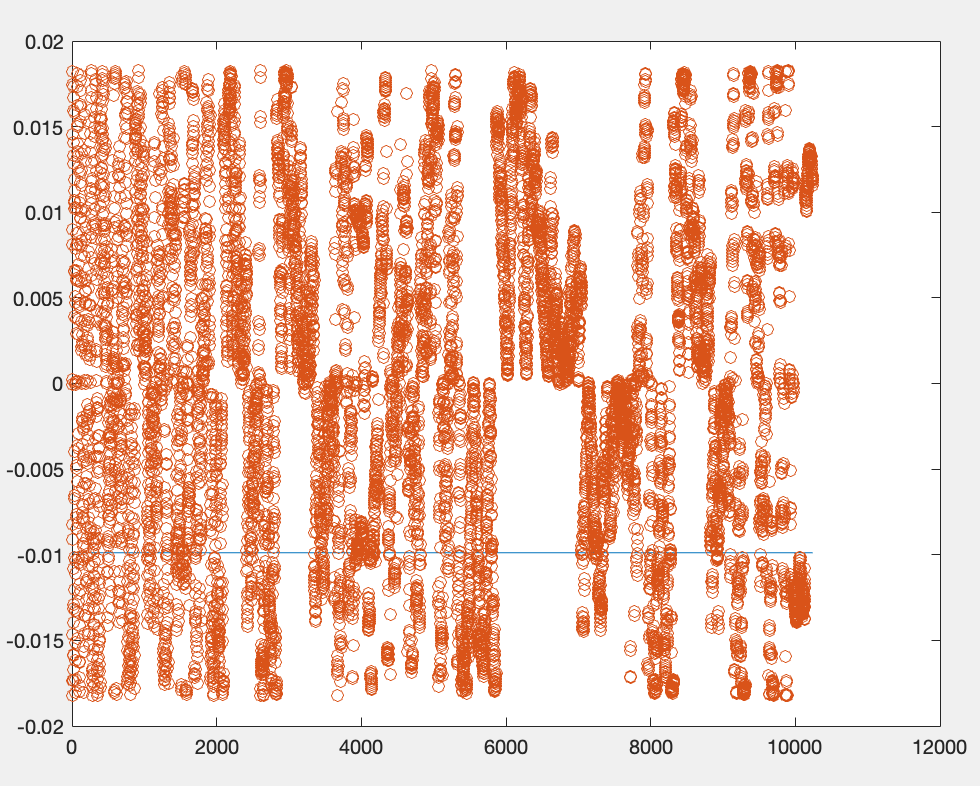
\includegraphics[width=\textwidth]{13.png}
            {{\small Entries of the eigenvectors associated with the first (blue) and second (red) smallest eigenvalues of the Laplacian matrix L for the graph ”crack.”}}    
        \end{subfigure}
        \hfill
        \begin{subfigure}[b]{0.475\textwidth}   
            \centering 
            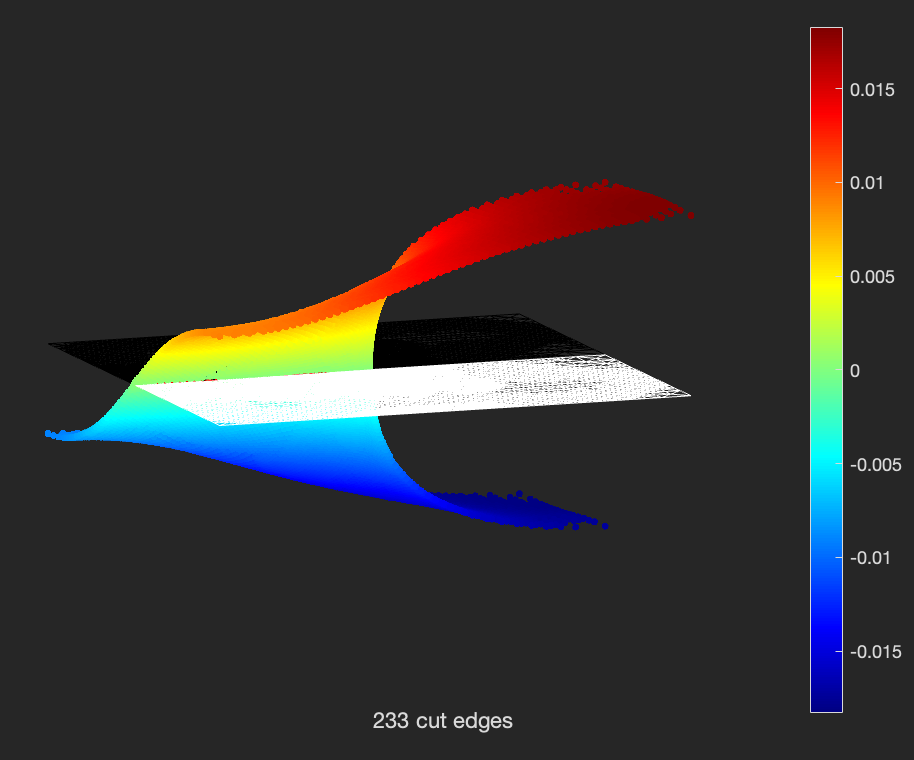
\includegraphics[width=\textwidth]{14.png}
            {{\small Projection of the entries of the eigenvector associated with the second smallest eigenvalue onto the coordinate system space of the graph ”crack.”}}    
        \end{subfigure}
\vskip\baselineskip
        \begin{subfigure}[b]{0.475\textwidth}   
            \centering 
            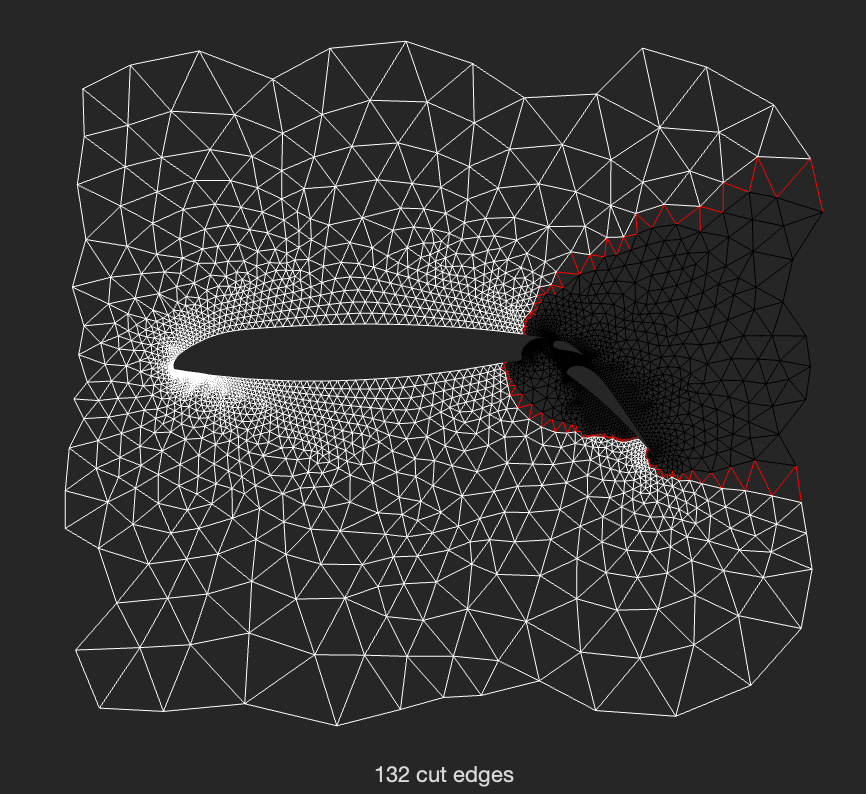
\includegraphics[width=\textwidth]{airfoil.png}
            {{\small "airfoil1" graph. Red are the cut edges of the mesh, while white is translated to light blue and black to yellow in the corresponding spectral coordinates graph.}}    
        \end{subfigure}
        \hfill
        \begin{subfigure}[b]{0.475\textwidth}   
            \centering 
            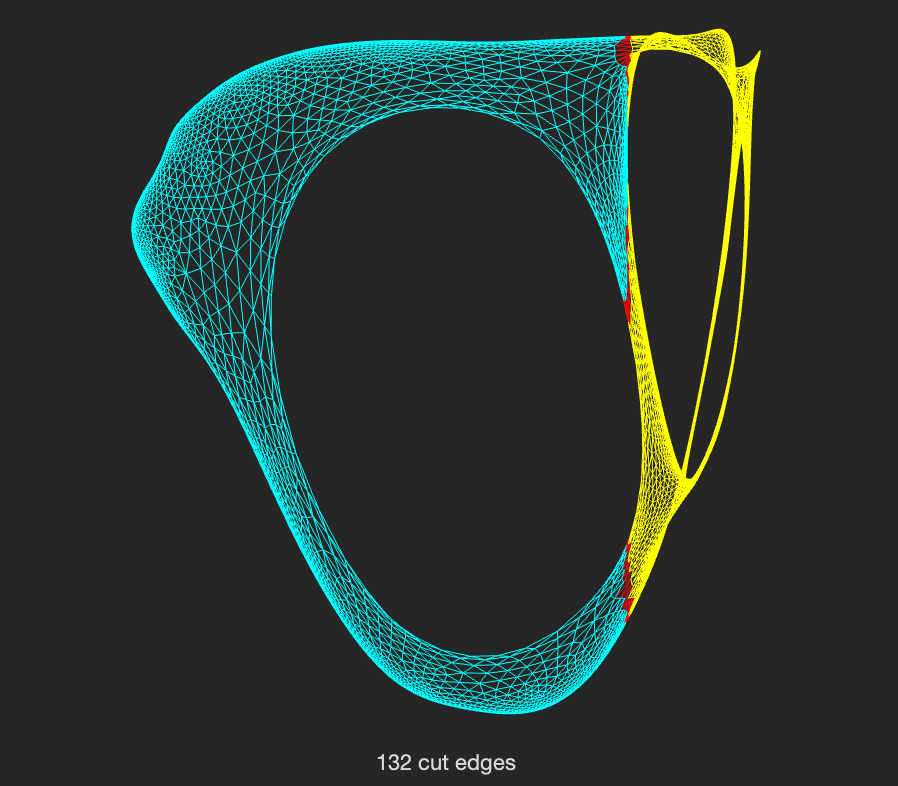
\includegraphics[width=\textwidth]{3.png}
            {{\small Spectral coordinates graph of the "airfoil1" mesh.  Light blue corresponds to white and black to yellow in the spatial coordinates graph.}}    
        \end{subfigure}
\label{figure:ex61meshes}
    \end{figure}

\begin{figure}[H]
        \centering
\begin{subfigure}[b]{0.475\textwidth}   
            \centering 
            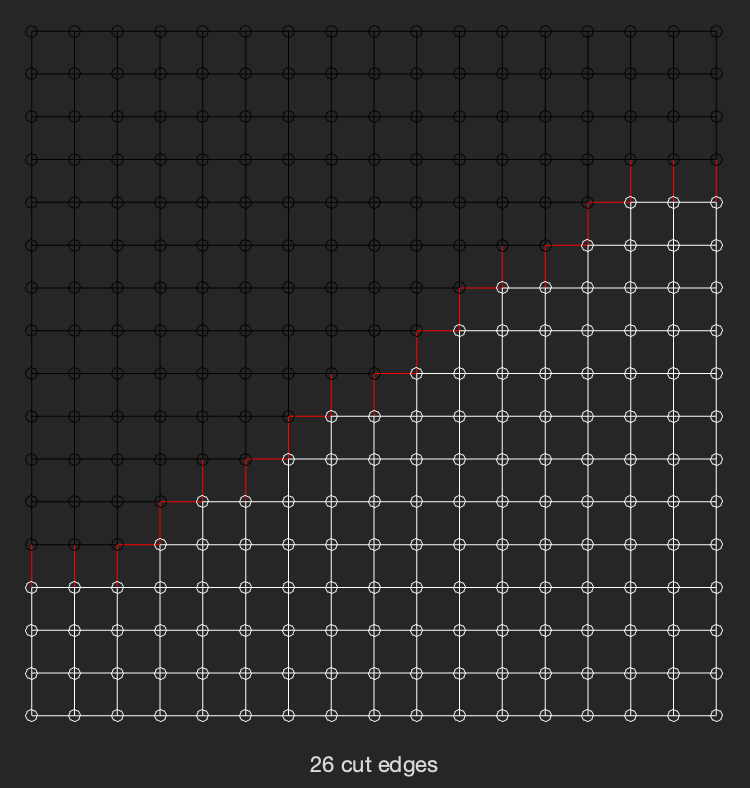
\includegraphics[width=\textwidth]{mesh3e1.png}
            {{\small "mesh3e1" graph. Red are the cut edges of the mesh, while white is translated to light blue and black to yellow in the corresponding spectral coordinates graph.}}    
        \end{subfigure}
        \hfill
        \begin{subfigure}[b]{0.475\textwidth}   
            \centering 
            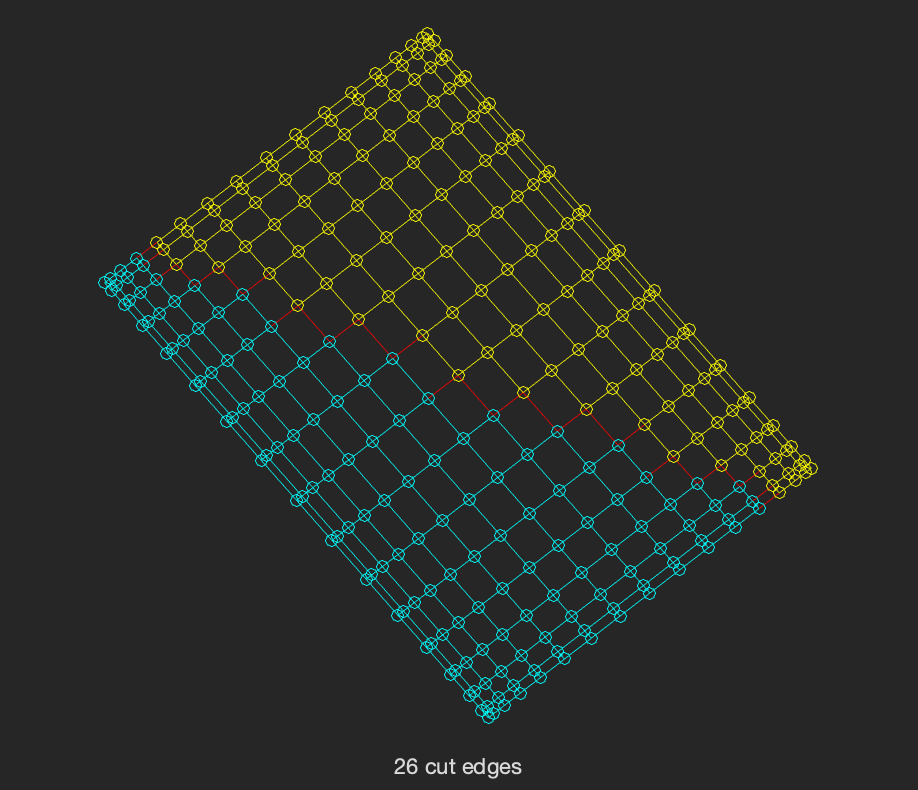
\includegraphics[width=\textwidth]{6.png}
            {{\small Spectral coordinates graph of the "mesh3e1" mesh.  Light blue corresponds to white and black to yellow in the spatial coordinates graph.}}    
        \end{subfigure}
\vskip\baselineskip
\begin{subfigure}[b]{0.475\textwidth}   
            \centering 
            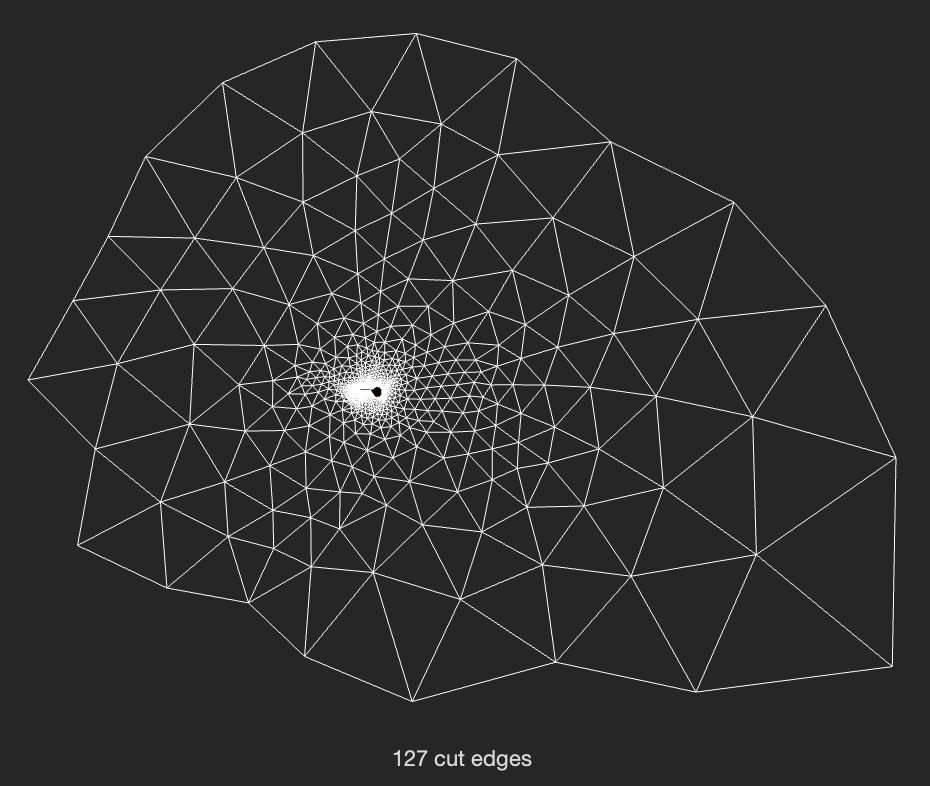
\includegraphics[width=\textwidth]{barth4.png}
            {{\small "barth4" graph. Red are the cut edges of the mesh, while white is translated to light blue and black to yellow in the corresponding spectral coordinates graph.}}    
        \end{subfigure}
        \hfill
        \begin{subfigure}[b]{0.475\textwidth}   
            \centering 
            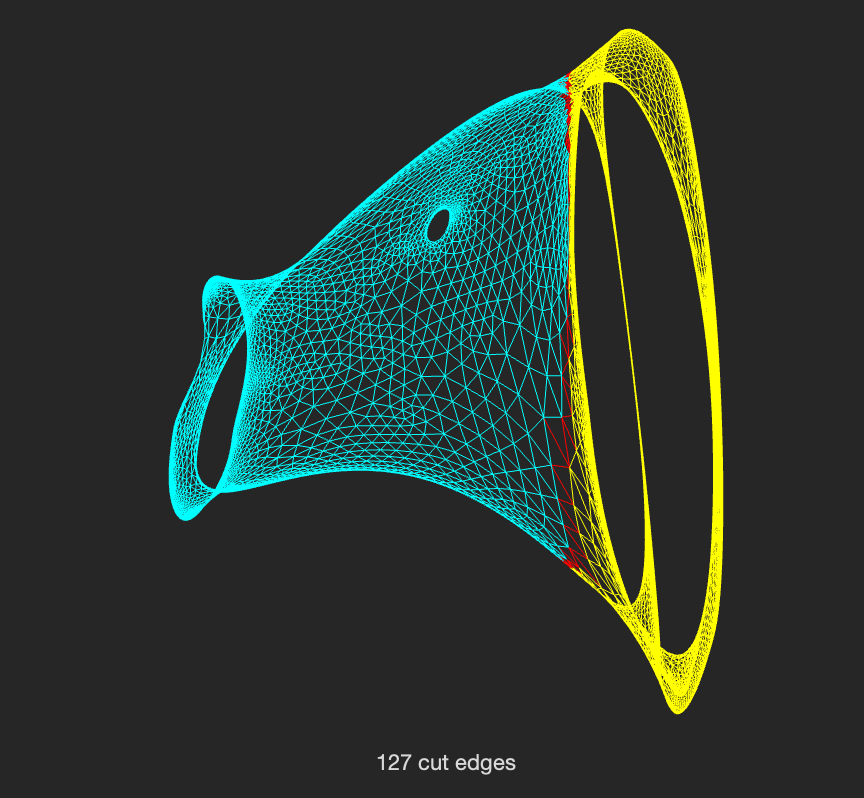
\includegraphics[width=\textwidth]{9.png}
            {{\small Spectral coordinates graph of the "barth4" mesh.  Light blue corresponds to white and black to yellow in the spatial coordinates graph.}}    
        \end{subfigure}
\label{figure:ex62meshes}
    \end{figure}

\begin{figure}[H]
\centering
        \begin{subfigure}[b]{0.475\textwidth}   
            \centering 
            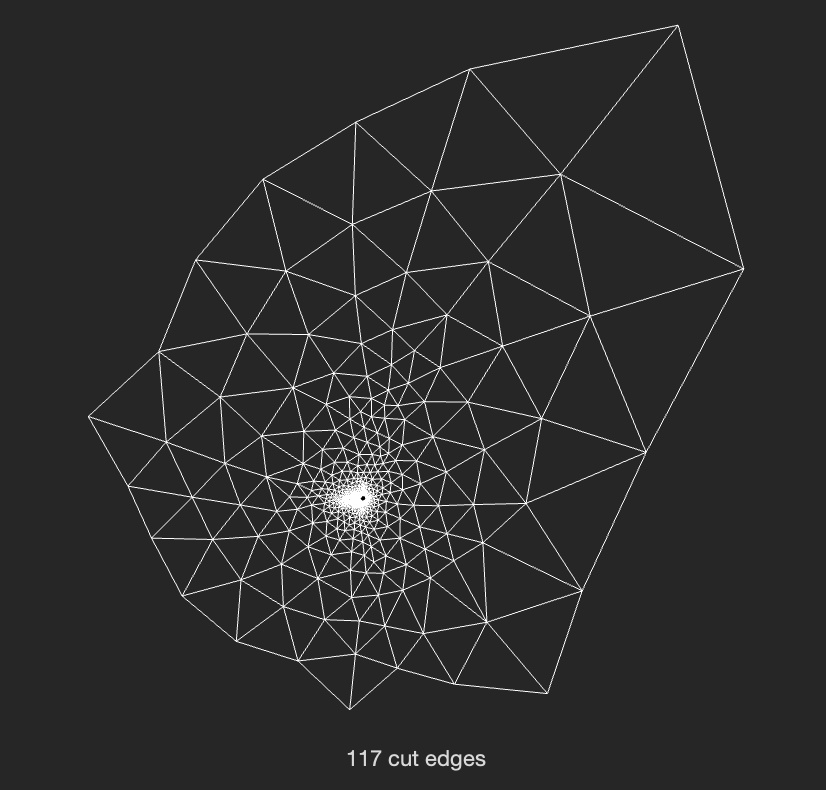
\includegraphics[width=\textwidth]{3elt.png}
            {{\small "3elt" graph. Red are the cut edges of the mesh, while white is translated to light blue and black to yellow in the corresponding spectral coordinates graph.}}    
        \end{subfigure}
        \hfill
        \begin{subfigure}[b]{0.475\textwidth}   
            \centering 
            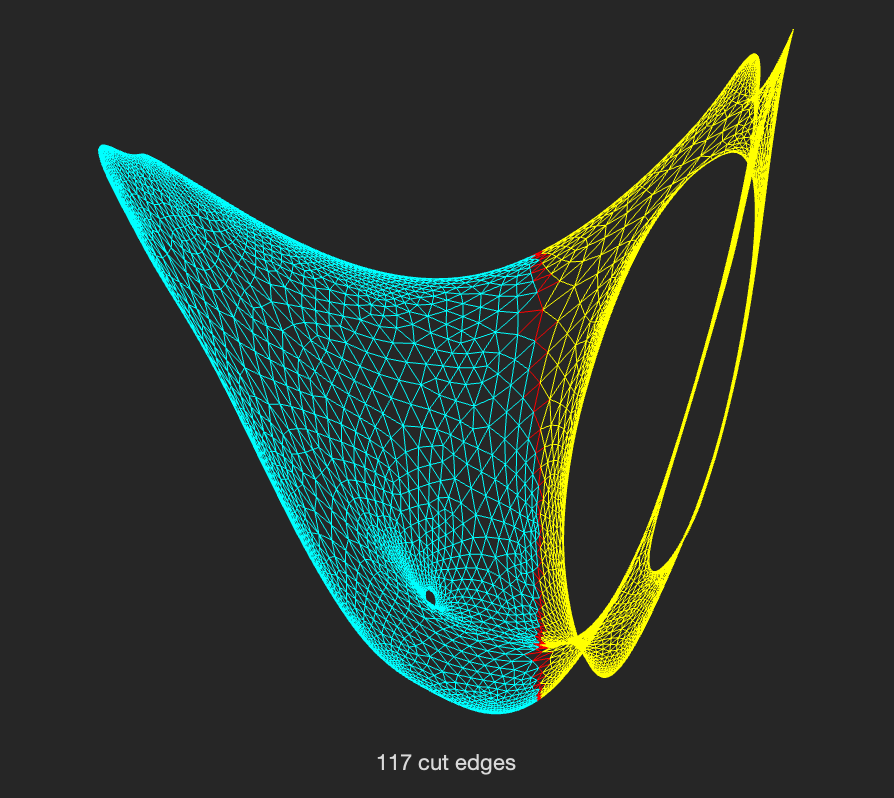
\includegraphics[width=\textwidth]{12.png}
            {{\small Spectral coordinates graph of the "3elt" mesh. Light blue corresponds to white and black to yellow in the spatial coordinates graph.}}    
        \end{subfigure}
\vskip\baselineskip
  \begin{subfigure}[b]{0.475\textwidth}   
            \centering 
            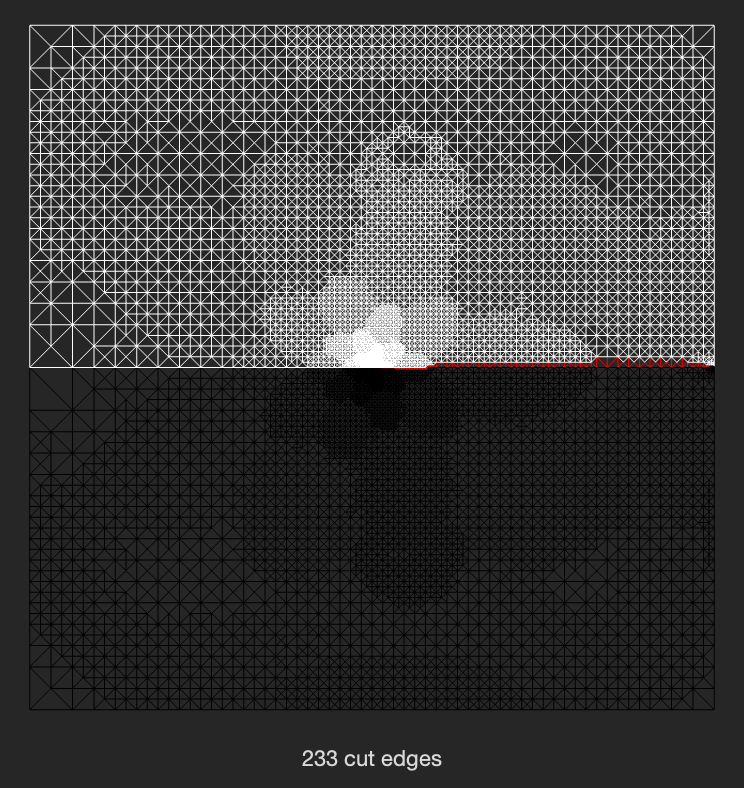
\includegraphics[width=\textwidth]{crack.png}
            {{\small "crack" graph. Red are the cut edges of the mesh, while white is translated to light blue and black to yellow in the corresponding spectral coordinates graph.}}    
        \end{subfigure}
        \hfill
        \begin{subfigure}[b]{0.475\textwidth}   
            \centering 
            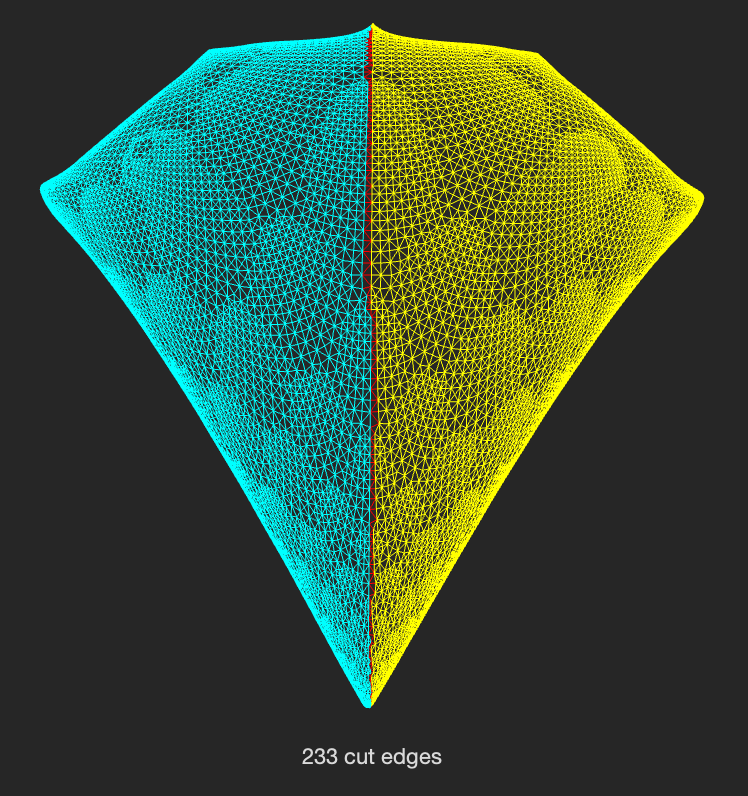
\includegraphics[width=\textwidth]{15.png}
            {{\small Spectral coordinates graph of the "crack" mesh.  Light blue corresponds to white and black to yellow in the spatial coordinates graph.}}    
        \end{subfigure}
\label{figure:ex63meshes}
    \end{figure}

\section{Task: Quality of the Report [15 Points] }


\end{document}
